\documentclass[doktyp=studarbeit]{TUBAFarbeiten}

\usepackage{selinput}% Auswahl der Dateikodierung (ansi,latin1,utf8,...)
\usepackage[T1]{fontenc}% Einstellung Fontencoding
\usepackage{amsmath}
\usepackage[section]{placeins}
%\usepackage{titlesec}
\usepackage{xcolor}
\usepackage{listings}
% \usepackage{hyperref}
\usepackage{csquotes}

\newcommand\tab[1][5mm]{\hspace*{#1}}
\newtheorem{thm}{Theorem}
\newtheorem{lem}[thm]{Lemma}
	\SelectInputMappings{adieresis={ä},germandbls={ß},Euro={€}}

% Packages for images and caption in figures
\usepackage{graphicx}
\graphicspath{ {./img/} }
\usepackage{subcaption}

\definecolor{mGreen}{rgb}{0,0.6,0}
\definecolor{mGray}{rgb}{0.5,0.5,0.5}
\definecolor{mPurple}{rgb}{0.58,0,0.82}
\definecolor{backgroundColour}{rgb}{0.95,0.95,0.92}

\lstdefinestyle{C++}{
    backgroundcolor=\color{backgroundColour},   
    commentstyle=\color{mGreen},
    keywordstyle=\color{magenta},
    numberstyle=\tiny\color{mGray},
    stringstyle=\color{mPurple},
    basicstyle=\footnotesize,
    breakatwhitespace=false,         
    breaklines=true,                 
    captionpos=b,                    
    keepspaces=true,                 
    numbers=left,                    
    numbersep=5pt,                  
    showspaces=false,                
    showstringspaces=false,
    showtabs=false,                  
    tabsize=2,
    language=C++
}

\usepackage[backend=biber,sortlocale=de_DE_phonebook]{biblatex}
\addbibresource{references.bib}

%\usepackage{setspace}% Einstellungen Zeilenabstand
	%\onehalfspacing% Einstellungen Zeilenabstand

\TUBAFFakultaet{Fakultät für Mathematik und Informatik}
\TUBAFInstitut{Institut für Informatik}

\TUBAFTitel[OpenGL Game: Achtung, die Kurve!]{OpenGL Game: Achtung, die Kurve!}
\TUBAFBetreuer{M.Sc. Jonas Treumer}
\TUBAFKorrektor{M.Sc. Ben Lorenz}
\TUBAFAutor[Al Nomer/Valdés]{Simon Al Nomer und Hernán Felipe Valdés González}
\TUBAFStudiengang{Bachelor Angewandte Informatik}
\TUBAFMatrikel{64\,082\newline 63\,952}
\TUBAFDatum[2020-10-19]{19. Oktober 2020}

\begin{document}

\maketitle

\TUBAFErklaerungsseite

%%%%%%%%%%%%%%%%%%%%%%%%%%%%%%%%%%%%%%%%%%%%%%%%%%%%%%%%%%%%%%%%%%%%%%%%%%%%%%%%
\addsec{Zusammenfassung}
Implementierung des Spieles ''Achtung, die Kurve'' in C++ mit OpenGL für die 
Lehreveranstaltung ''Multimedia''.

%%%%%%%%%%%%%%%%%%%%%%%%%%%%%%%%%%%%%%%%%%%%%%%%%%%%%%%%%%%%%%%%%%%%%%%%%%%%%%%%


\KOMAoptions{
	listof=totoc	% Abbildungs- und Tabellenverzeichnis im Inhaltsverzeichnis
}

\tableofcontents
% \listoffigures
% \listoftables

\newpage

\section{Einführung}

Achtung, Die Kurve ist ein Multiplayer-Spiel, welches im Jahr 1995 von 
Filip Oščádal und Kamil Doležal in DOS entwickelt wurde. Im Jahr 2010 wurde 
eine neue Version des Spiels unter dem Namen “Achtung, die Kurve! Flash Remake”
veröffentlicht. Diese Version ist mit Adobe Flash von Geert van den Burg 
entwickelt worden. Das Spiel kann von mehreren Spielern an einem Computer online gespielt werden.

Nachdem das Spiel großen Zuspruch fand, beschloss van den Burg, sich mit 
Robin Brouns zusammenzuschließen und eine Fortsetzung zu entwickeln, welche 
2011 unter den Namen Curve Fever (Originaltitel “Achtung, die Kurve! 2”) 
veröffentlicht. Es kann online und mit Spielern aus dem Netz gespielt werden.

In den folgenden Jahren wurden dem Spiel immer weiter neue Features 
hinzugefügt wie zum Beispiel verschiedene Boni, die Möglichkeit, in einem Team 
zu spielen, oder das Bestehen einer Rangliste.

2015 sammelte van den Burg ein Team um sich, um eine neue Version des Spiels in 
HTML5 zu implementieren, welche im September 2016 auf dem Markt kam.

\begin{figure}[!htb]
    \centering
    \begin{subfigure}[b]{0.45\textwidth}
		\centering
        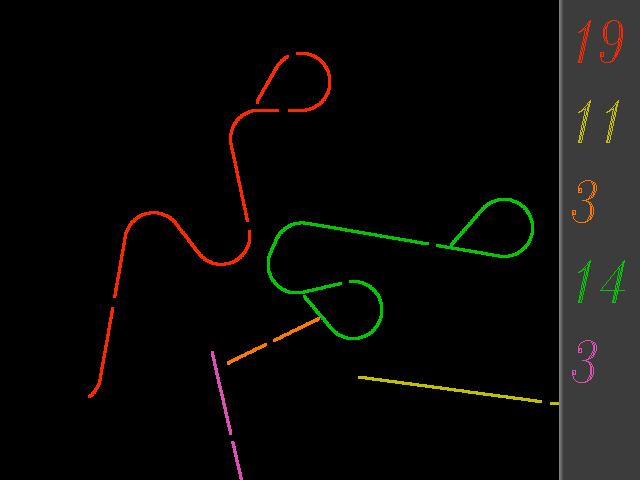
\includegraphics[width=1\linewidth]{dos-version.png}
		\caption{Original version für DOS (1995).}
	\end{subfigure}
	\qquad
	\begin{subfigure}[b]{0.45\textwidth}
		\centering
        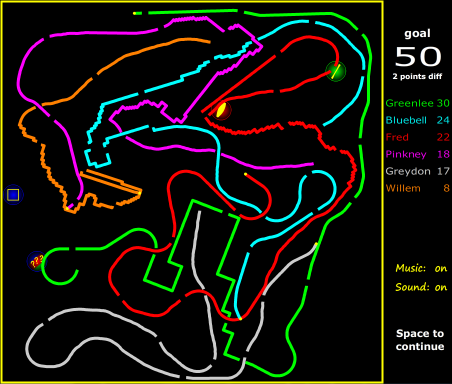
\includegraphics[width=1\linewidth]{flash-version.png}
        \caption{Flash remake (2010).}
	\end{subfigure}
    \caption{2 Versionen, die als Basis für das Spiel genommen wurden.}
	\label{fig:dos-version}
\end{figure}

Die Implementierung unseres Spiels basiert auf die Version von 1995 in 
Kombination mit dem Stil der Flash Version.

\subsection{Spielmechanik}

Das Spiel können bis zu 6 Spieler zusammen an einem Bildschirm und mit einer 
Tastatur spielen. Jeder Spieler besitzt zwei vorbestimmten Tasten, die rechts 
und links symbolisieren. Um das Spiel zu starten, müssen mindestens 
2 Spieler spielen. Das Ziel des Spiels ist es, dass ein Spieler solange wie
möglich am Leben bleibt.

Jeder Spieler wird durch einen Kreis dargestellt, der mit jeder Bewegung einen 
Pfad mit seiner Farbe hinterlässt. Der Spieler kann sich nur nach
rechts oder links drehen und damit die Richtung seiner Bewegung ändern. Wenn
der Spieler nicht reagiert, bewegt er sich weiter in die gleiche Richtung.

Ein Spieler verliert, wenn er gegen seine eigene Linie, die Linie anderen 
Spieler oder den Rand stößt. Das Spiel ist zu Ende, wenn nur noch ein 
Spieler am Leben ist.

\section{Softwaredokumentation}

Unseres Projekt hat den Code als Basis, der zusammen während der Vorlesung 
erstellt wurde. Dieser Code wurde in C++ migriert. 
Die Entscheidung, das Spiel in C++ statt in C zu programmieren, lag 
insbesondere an der Standardbibliothek von C++ und deren implementierten 
Daten-Strukturen sowie die Eigenschaft mit Klassen zu programmieren.

Für die Softwarearchitektur wurde das State Pattern implementiert, um einen 
endlichen Automaten zu simulieren. Die Änderungen der Zuständen sind in der 
Klasse \textit{Game} durchgeführt.

Das Spiel wurde im Sinne von Szenen programmiert. Die Klasse \textit{Game}
verhält sich als eine Szene sowie als eine Szene-Manager. Die anderen
zwei Szenen sind \textit{Menu} und \textit{GameOver}.

In dem Spiel wird zwischen User und Player differenziert. Das Spiel besitzt nur
ein User, der die Kontrolle über den Computer besitzt und mehrere Player, 
welche die Kreise kontrollieren.

\subsection{user\_data\_t}

Die Daten des laufenden Spiels, sowie die Anzahl an Spieler und ihren Punkten
werden in einem Struct gespeichert, der dann in GLFW zur Verfügung gestellt wird.
Dieser Struct heißt \textit{user\_data\_t}.

\begin{lstlisting}[style=C++]
typedef struct {
    int window_width;
    int window_height;
    GameState game_state;
    std::vector<player_info_t>* player_info;
} user_data_t;
\end{lstlisting}

\subsection{player\_info}
Alle Player werden am Anfang des Programmes in main.cpp addiert und dann
im Menü als aktiv gesetzt.

\begin{lstlisting}[style=C++]
typedef struct {
    bool is_active;
    int id;
    std::string name;
    std::string menu_text;
    Control control;
    std::array<GLubyte, 3> color;
    glm::vec3 menu_color;
    int score;
} player_info_t;
\end{lstlisting}

\subsection{Game}

\begin{figure}
    \centering
    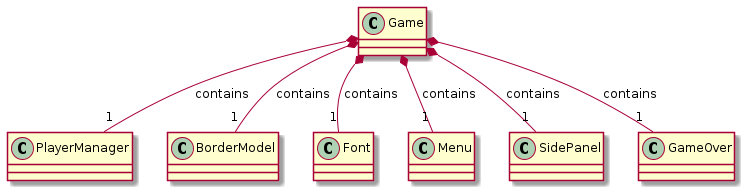
\includegraphics[width=0.9\linewidth]{Game.png}
	\caption{UML Diagramm von der Klasse Game}
	\label{fig:game-uml}
\end{figure}

Die zentrale Klasse des Projektes ist \textit{Game}. In dieser Klasse 
werden die Zustände des Automaten geändert und unterschiedliche Klassen 
initialisiert und geteilt. In der Abb. \ref{fig:game-uml} steht die 
Klassen, die anschließend im \textit{Game} initialisiert werden. 
Ein Beispiel ist die Klasse \textit{Font}, die für die Erzeugung und für die
Zeichnung von Texten verantwortlich ist. Sie wird nur einmal in \textit{Game}
initialisiert und im Folgenden mit anderen Klassen geteilt.  

\FloatBarrier
\subsection{GameState}

In der Abb. \ref{fig:state-machine} wird der Automat des Spieles dargestellt. 
Der Startzustand des Automaten ist GAME\_MENU. 

\begin{figure}
    \centering
    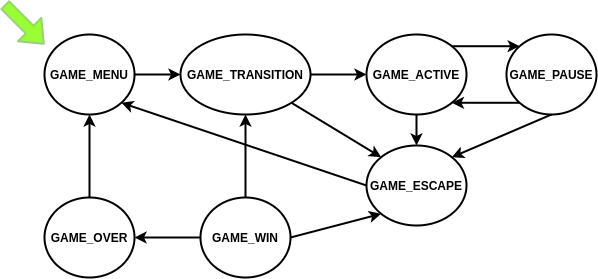
\includegraphics[width=0.7\linewidth]{state_machine.png}
	\caption{Darstellung des Zustandsautomaten}
	\label{fig:state-machine}
\end{figure}

\paragraph{GAME\_MENU}
Es wird das Menü für den Auswahl von Spielern gezeigt. Es kann nur zu dem
nächsten Zustand übergegangen werden (GAME\_TRANSITION), in dem mindestens 
2 Spieler
ihre Anwesenheit bestätigen und dann die SPACE-Taste gedrückt wird.
\paragraph{GAME\_TRANSITION}
Das Spiel ist bereit, zu starten. Alle Spieler sind auf ihren Plätzen und ihre
Positionen werden mit einem gefärbten Kreis gezeichnet. Um das Spiel zu starten,
muss die SPACE-Taste gedrückt werden und der neuer Zustand wird GAME\_ACTIVE. 
Um zurück ins Menü zu gehen, muss die ESCAPE-Taste gedrück werden und 
der neuer Zustand wird GAME\_ESCAPE.
\paragraph{GAME\_ACTIVE}
Das Spiel läuft und die Spieler dürfen anderen umschließen und in die Irre führen.
Es kann in jedem Moment die SPACE-Taste gedrückt werden, um das Spiel zu pausieren
und der neuer Zustand wird GAME\_PAUSE. Es kann auch mit der ESCAPE-Taste das
Spiel abgebrochen und zurück ins Menü gelangt werden. Dann wird der 
neue Zustand GAME\_ESCAPE. 
Wenn nur ein Spieler auf dem Feld übrig ist, wird der Zustand
automatisch zu GAME\_WIN oder GAME\_OVER übergehen, abhängig ob die maximale 
Punktzahl erreicht wurde oder nicht.
\paragraph{GAME\_PAUSE}
Das Spiel ist pausiert. Mit der SPACE-Taste kann zurück zu GAME\_ACTIVE 
und mit der ESCAPE-Taste zu GAME\_ESCAPE übergegangen werden.
\paragraph{GAME\_ESCAPE}
ist ein Zwischenzustand, welcher die Daten wieder ins Default 
bringt. Es wird direkt zu GAME\_MENU gegangen.
\paragraph{GAME\_WIN}
ist ein Zwischenzustand, der den Gewinner der Runde anzeigt 
(mit einem blinkenden Namen).
Nach ein paar Frames wird direkt zu GAME\_TRANSITION gegangen, um eine 
neue Runde zu starten. 
\paragraph{GAME\_OVER}
Es wird eine Liste mit der gesamten Punktzahl angezeigt. Wird die SPACE-Taste
gedrückt, erscheint das GAME\_MENU und alles startet von vorne.

\subsection{Model und Mesh}
Die Klassen \textit{Model} und \textit{Mesh} sind zwei abstrakte Klassen, welche
als Basisklasse angewandt werden.

\paragraph{Mesh} 
Ein \textit{Mesh} enthält die Punkte, die gezeichnet werden, das 
Vertex Array Object (VAO) und das Vertex Buffer Object (VBO). 
Die Klassen \textit{BorderMesh}, \textit{PlayerMesh} und \textit{LineMesh} 
erben vom \textit{Mesh}. Diese Klassen müssen die Funktion ''draw'' deklarieren,
um die Punkte zu zeichnen.

\paragraph{Model} 
Ein \textit{Model} enthält ein \textit{Mesh} und die ID des \textit{Shader},
welches angewandt wird. Ein \textit{Model} interagiert mit \textit{Game}. In
dieser Klasse werden die Positionen und Transformation durch die Funktion 
''update'' informiert.

\subsection{Display}

Die Klasse \textit{Display} initialisiert und besitzt eine Instanz von GLFWwindow. 
Ein Pointer des Fensters wird dann an die Klasse \textit{Game} übergeben. 
Anschließend schließt \textit{Display} am Ende des Programms auch das Fenster 
(beenden).

Das Fenster hat eine ursprüngliche Ratio von 1:1 mit einer Größe von 700x700 Pixel.
Das Fenster behält sein Aspect Ratio, indem es immer den kleinsten Wert 
zwischen Höhe und Breite nimmt und sich dann in der Mitte positioniert. Ist zum Beispiel die Höhe größer als die Breite, zentriert das 
Fenster sich in der Mitte von der Höhe mit der Größe von der Breite. Der Rest
wird mit einem schwarzen Padding gefüllt.

\begin{figure}[!htb]
    \centering
    \begin{subfigure}[b]{0.55\textwidth}
        \centering
        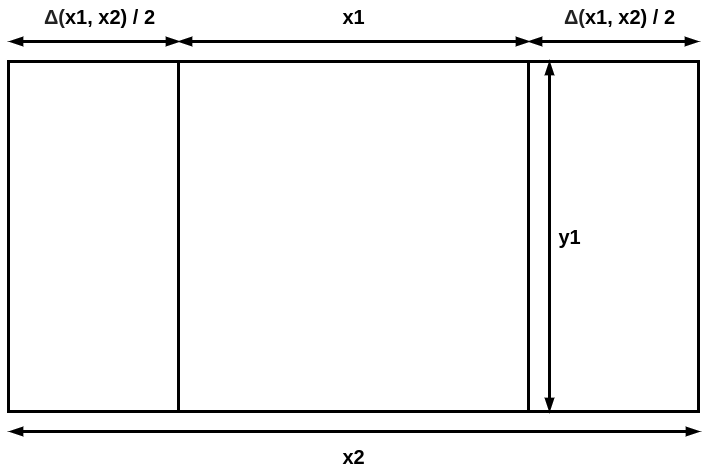
\includegraphics[width=1\linewidth]{display-2.png}
        \caption{Anpassung in horizontellen Resize}
    \end{subfigure}
    \begin{subfigure}[b]{0.4\textwidth}
        \centering
        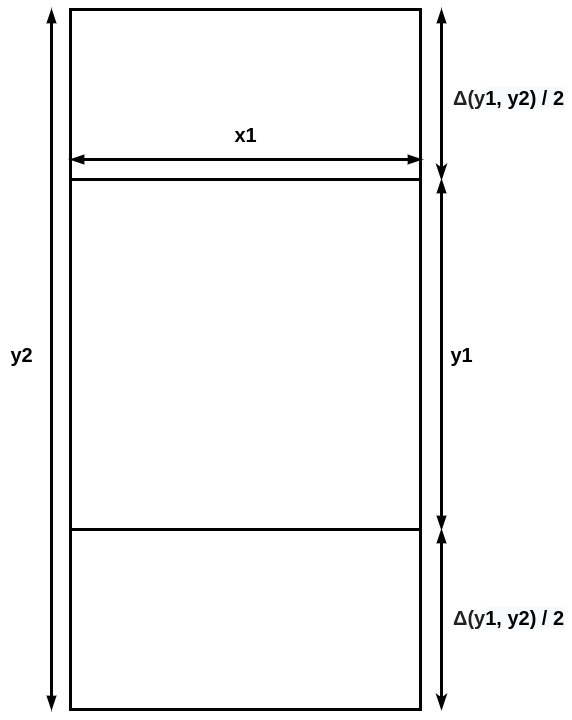
\includegraphics[width=1\linewidth]{display-3.png}
        \caption{Anpassung in vertikallen Resize}
    \end{subfigure}
    \caption{Anpassungen bei der Änderung in der Größe des Fensters}
	\label{fig:display}
\end{figure}

\begin{figure}[!htb]
    \centering
    \begin{subfigure}[b]{0.517\textwidth}
        \centering
        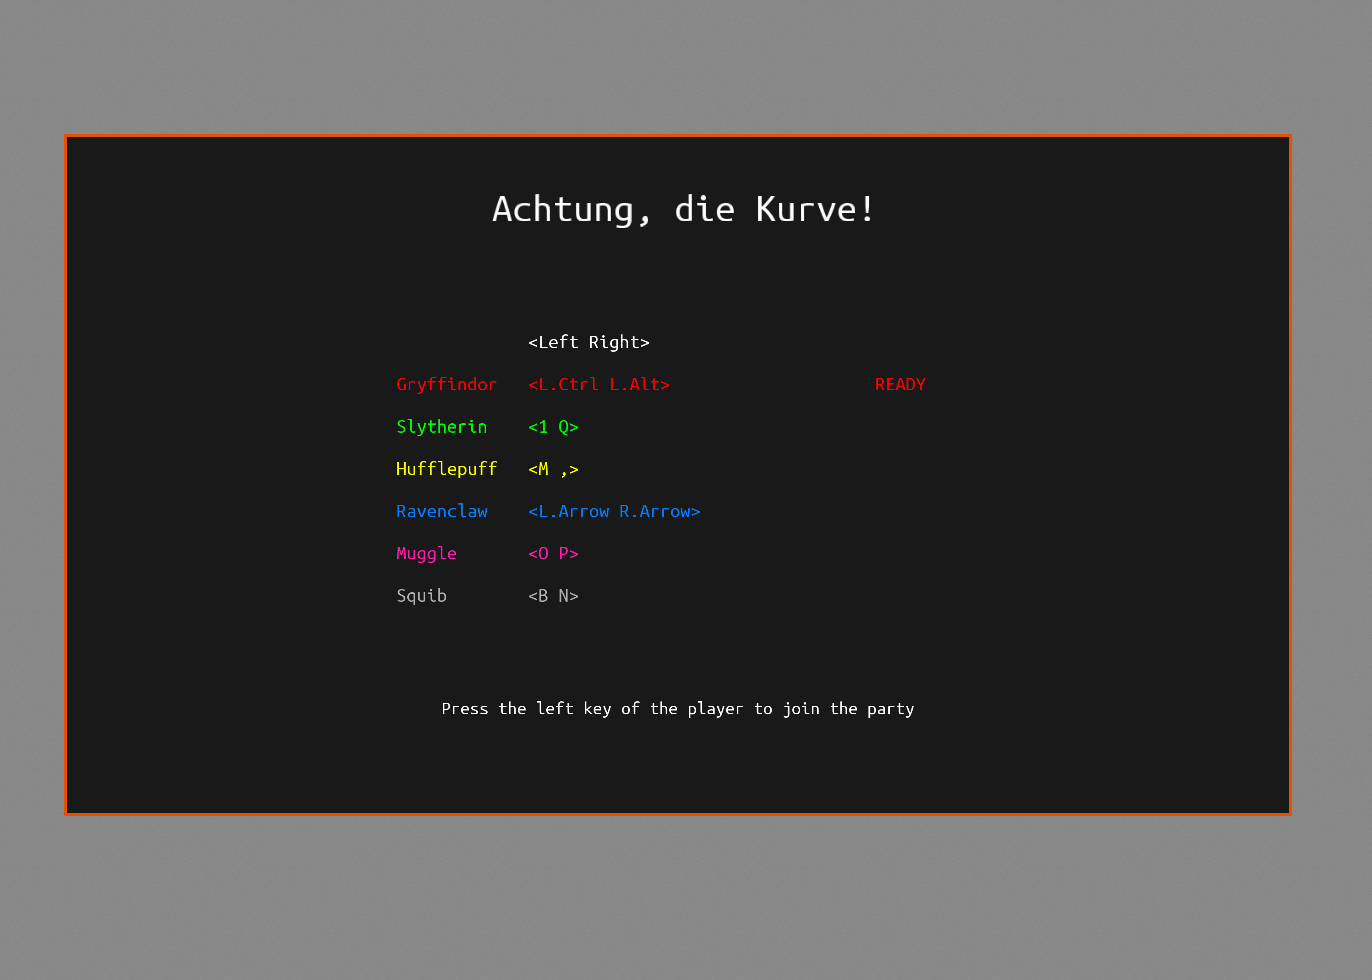
\includegraphics[width=1\linewidth]{aspect-ratio-1.png}
        \caption{Erstellung von den Punkten mit der Kreis-Gleichung}
    \end{subfigure}
    \begin{subfigure}[b]{0.45\textwidth}
        \centering
        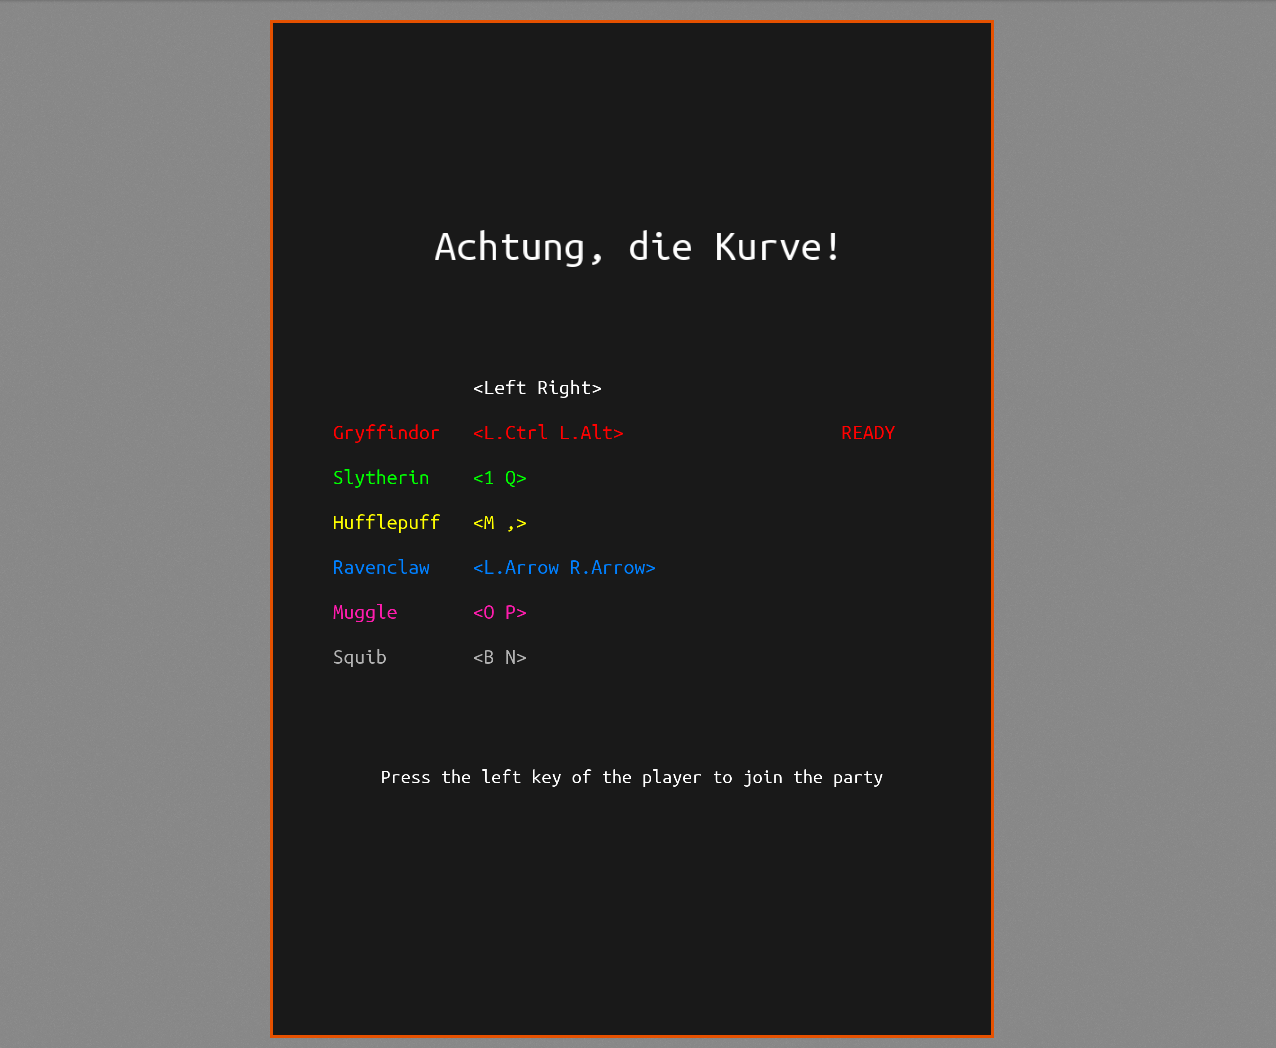
\includegraphics[width=1\linewidth]{aspect-ratio-2.png}
        \caption{Darstellung von GL\_TRIANGLE\_STRIP}
    \end{subfigure}
    \caption{Screenshots von dem Beispiel beim Resizing}
	\label{fig:display-aspect-ratio}
\end{figure}

\FloatBarrier
\subsection{Font}
Für die Erstellung von Texten ist in Anlehnung an einem Tutorial \cite{learn-opengl}.
Der Code wurde für das Projekt adaptiert. 
Die Lösung basiert auf die Bibliothek FreeType. FreeType ist in der Lage,
Schriftarten zu laden, Bitmap zu rendern und unterstützt mehrere Text-Operationen.


\section{Zeichnungen}

\subsection{Player}

\begin{figure}[!h]
    \centering
    \begin{subfigure}[b]{0.4\textwidth}
        \centering
        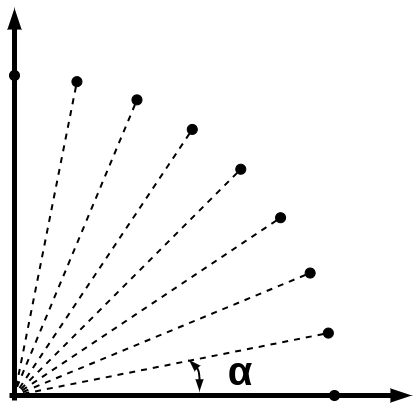
\includegraphics[width=0.8\linewidth]{kreis-1.png}
        \caption{Erstellung von den Punkten mit der Kreis-Gleichung}
    \end{subfigure}
    \begin{subfigure}[b]{0.4\textwidth}
        \centering
        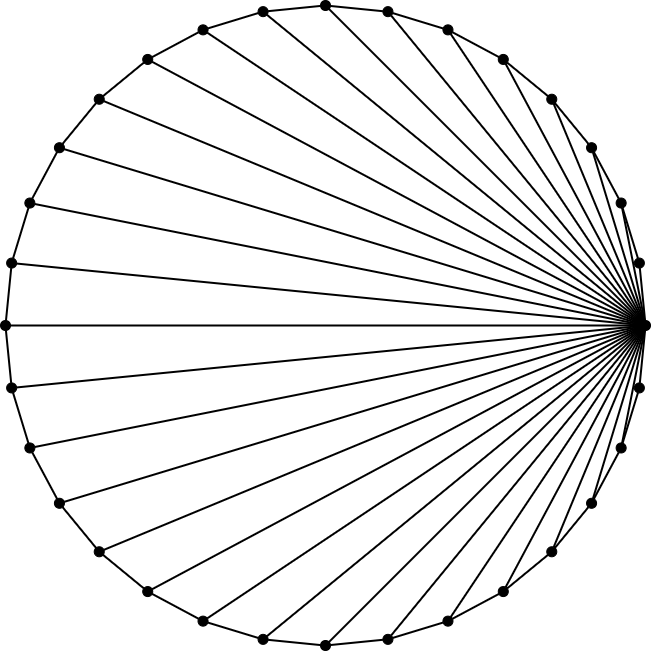
\includegraphics[width=0.8\linewidth]{kreis-2.png}
        \caption{Darstellung von GL\_TRIANGLE\_STRIP}
    \end{subfigure}
    \caption{Darstellung der Erstellung eines Kreises}
    \label{fig:player}
\end{figure}

Wie bereits anfangs erwähnt, wird jeder Spieler durch einen Kreis dargestellt. 
Die Erstellung der Kreise erfolgt durch Randpunkte des Kreises, welche den gleichen Radius zum Mittelpunkt haben. Diese Randpunkte werden durch die Funktion OpenGL Flag GL\_TRIANGLE\_STRIP verbunden. Eine Darstellung des Prozesses
ist in der Abb. \ref{fig:player} gezeigt.

\subsection{Linien}

Für das Zeichnen dicker Linien wurde ein Algorithmus entwickelt, der
in der Abb. \ref{fig:line-alg} dargestellt ist. 

Um den Winkel zwischen zwei Vektoren zu berechnen wurde die folgende 
trigonometrische Eigenschaft angewandt:

\begin{equation}
    cos(\theta)=
    \frac{\vec{v}_{1} \cdot \vec{v}_{2}}{
        \lVert \vec{v}_{1} \rVert 
        \lVert \vec{v}_{2} \rVert
    }
\end{equation}

Für die Drehrichtung der Linie wurde die z-Komponente des
Kreuzproduktes zwischen $\vec{v}_{1}$ und $\vec{v}_{2}$ analysiert.

\begin{equation}
    \vec{v}_{3} = \vec{v}_{1} \times \vec{v}_{2}
\end{equation}

Es gibt 3 Fälle:
\begin{enumerate}
    \item $\vec{v}_{3z}$ > 0: Die Linie dreht sich nach links
    \item $\vec{v}_{3z}$ < 0: Die Linie dreht sich nach rechts
    \item $\vec{v}_{3z}$ = 0: Die Linie ist gerade
\end{enumerate}

Wenn die neuen Punkte $L$ und $R$ berechnet wurden, können sie in dem LineMesh
hinzugefügt werden.
In der Abb. \ref{fig:line} ist eine graphische Darstellung des Algorithmus dargestellt.

\begin{figure}[!htb]
    \centering
    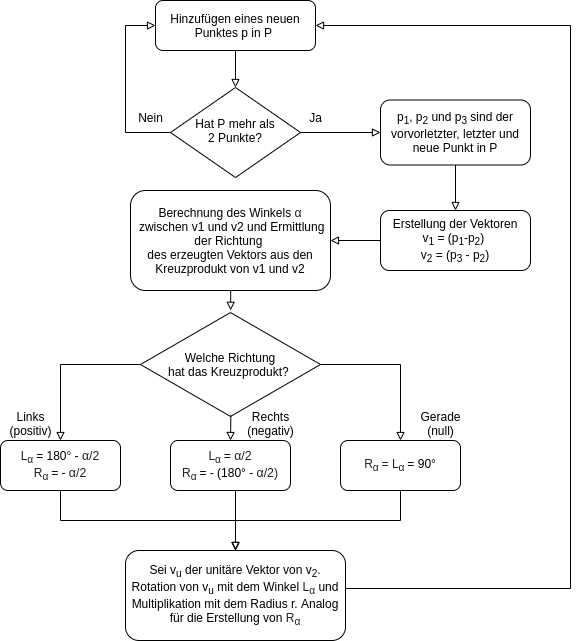
\includegraphics[width=0.8\linewidth]{line.png}
    \caption{Flow-Diagramm von der Linien-Erzeugung Algorithmus}
    \label{fig:line-alg}
\end{figure}

\begin{figure}[!htb]
    \centering
    \begin{subfigure}[b]{0.35\textwidth}
        \centering
        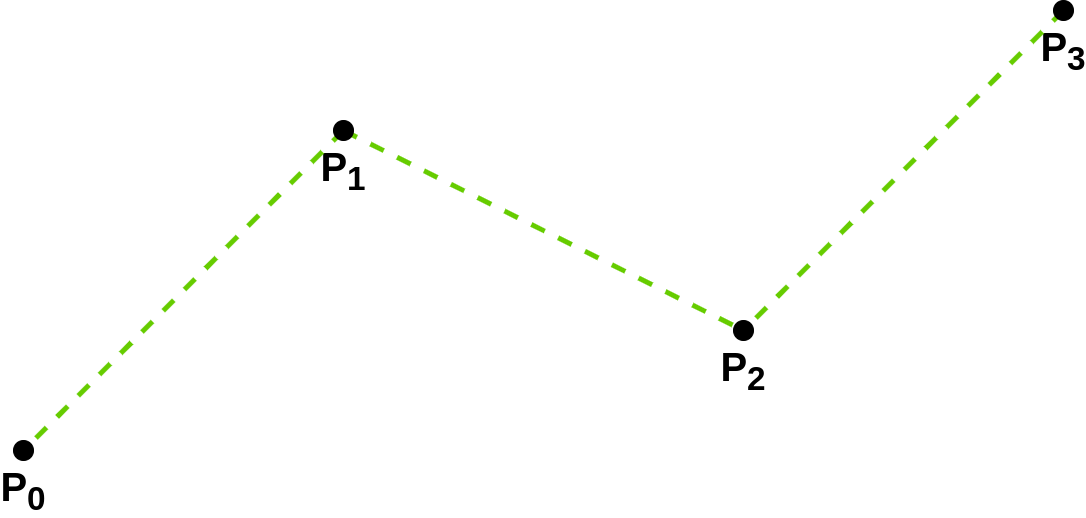
\includegraphics[width=1\linewidth]{Schlangenlinie-1.png}
        \caption{ursprünglichen Positionen des Players}
    \end{subfigure}
    \qquad
    \begin{subfigure}[b]{0.35\textwidth}
        \centering
        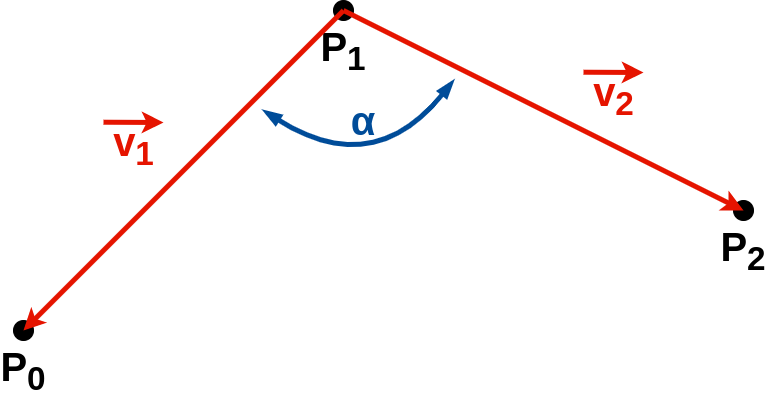
\includegraphics[width=1\linewidth]{Schlangenlinie-2.png}
        \caption{Erstellung von Vektoren und Berechnung ihren Winkel}
    \end{subfigure}
    \qquad
    \begin{subfigure}[b]{0.35\textwidth}
        \centering
        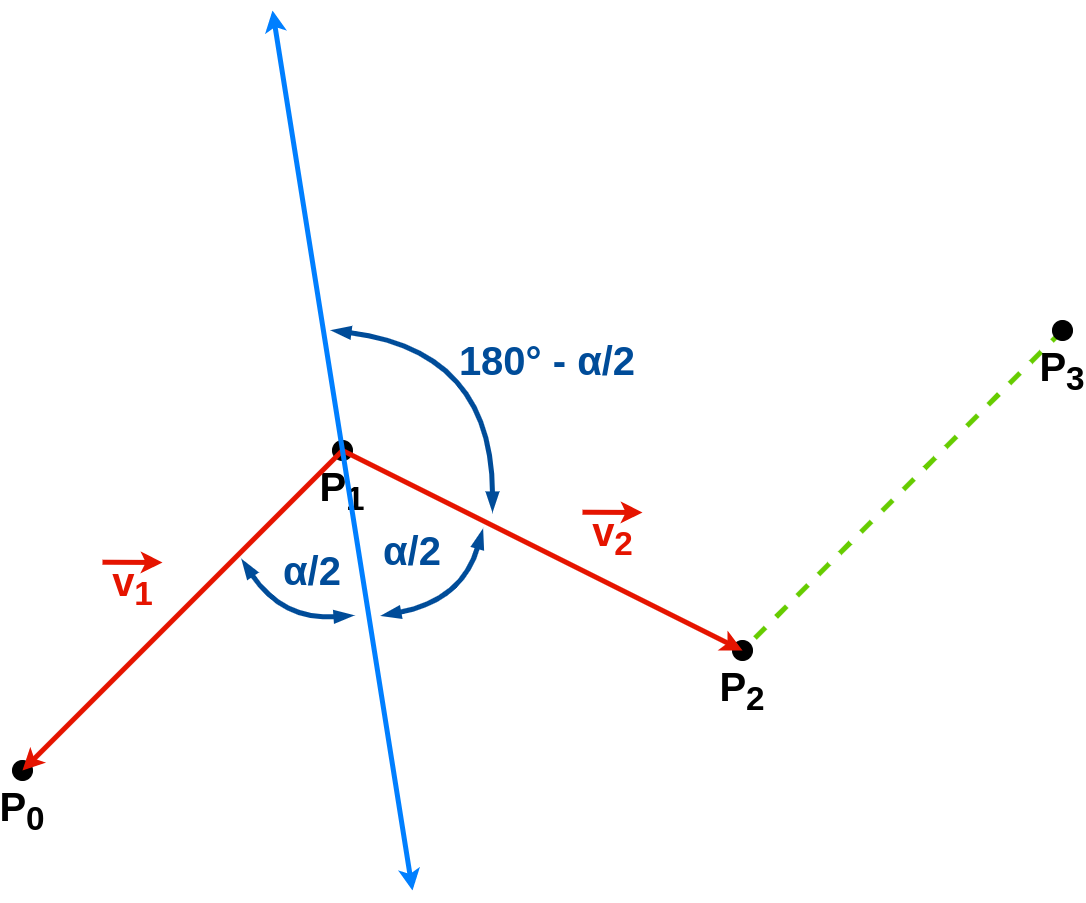
\includegraphics[width=1\linewidth]{Schlangenlinie-3.png}
        \caption{Schritt 3}
    \end{subfigure}
    \qquad
    \begin{subfigure}[b]{0.35\textwidth}
        \centering
        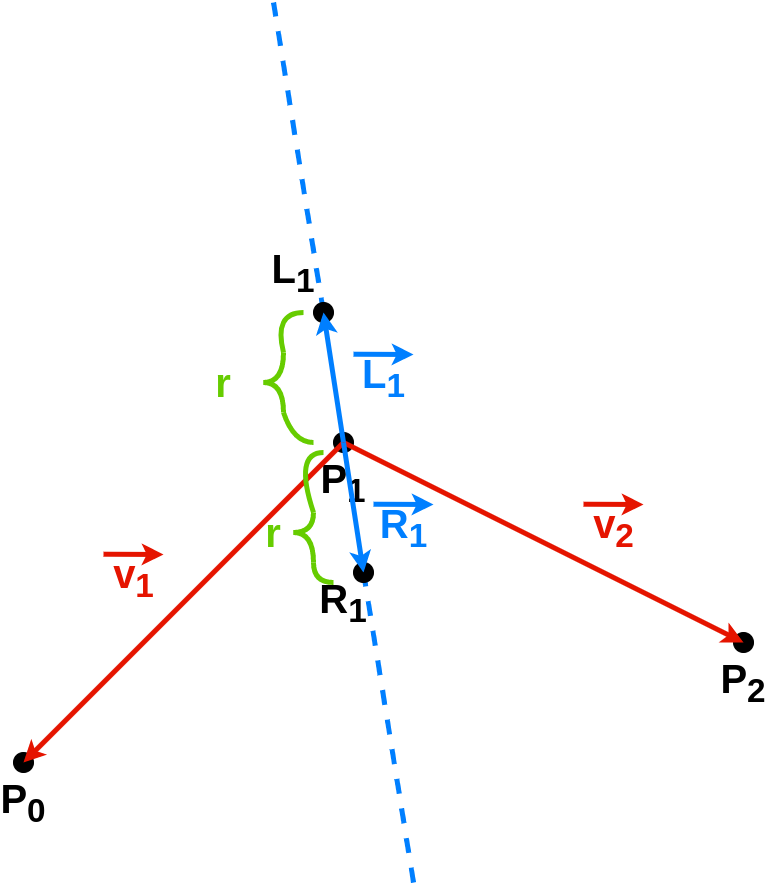
\includegraphics[width=1\linewidth]{Schlangenlinie-4.png}
        \caption{Schritt 4}
    \end{subfigure}
    \qquad
    \begin{subfigure}[b]{0.35\textwidth}
        \centering
        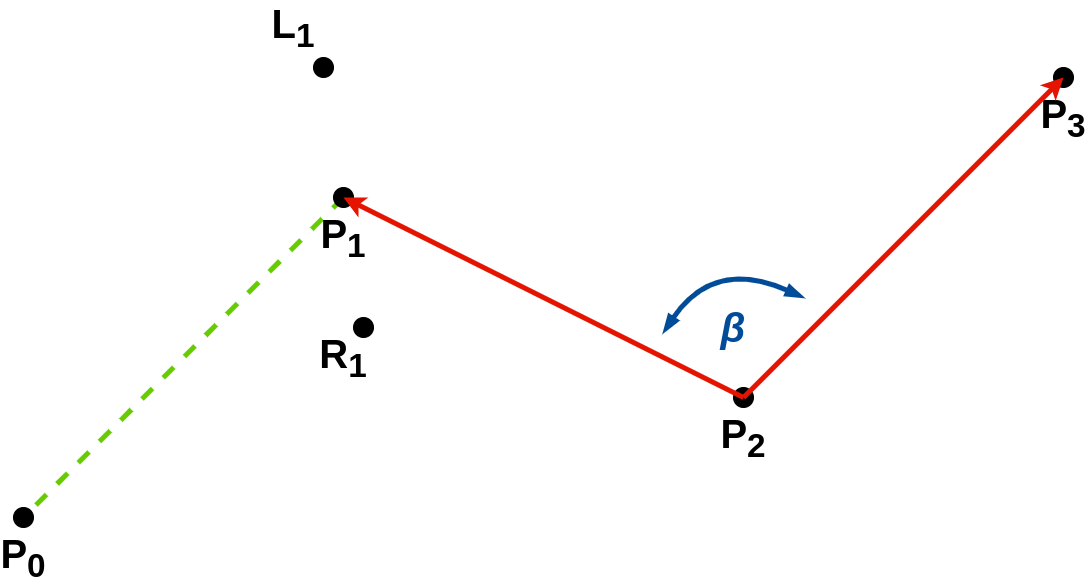
\includegraphics[width=1\linewidth]{Schlangenlinie-5.png}
        \caption{Schritt 5}
    \end{subfigure}
    \qquad
    \begin{subfigure}[b]{0.35\textwidth}
        \centering
        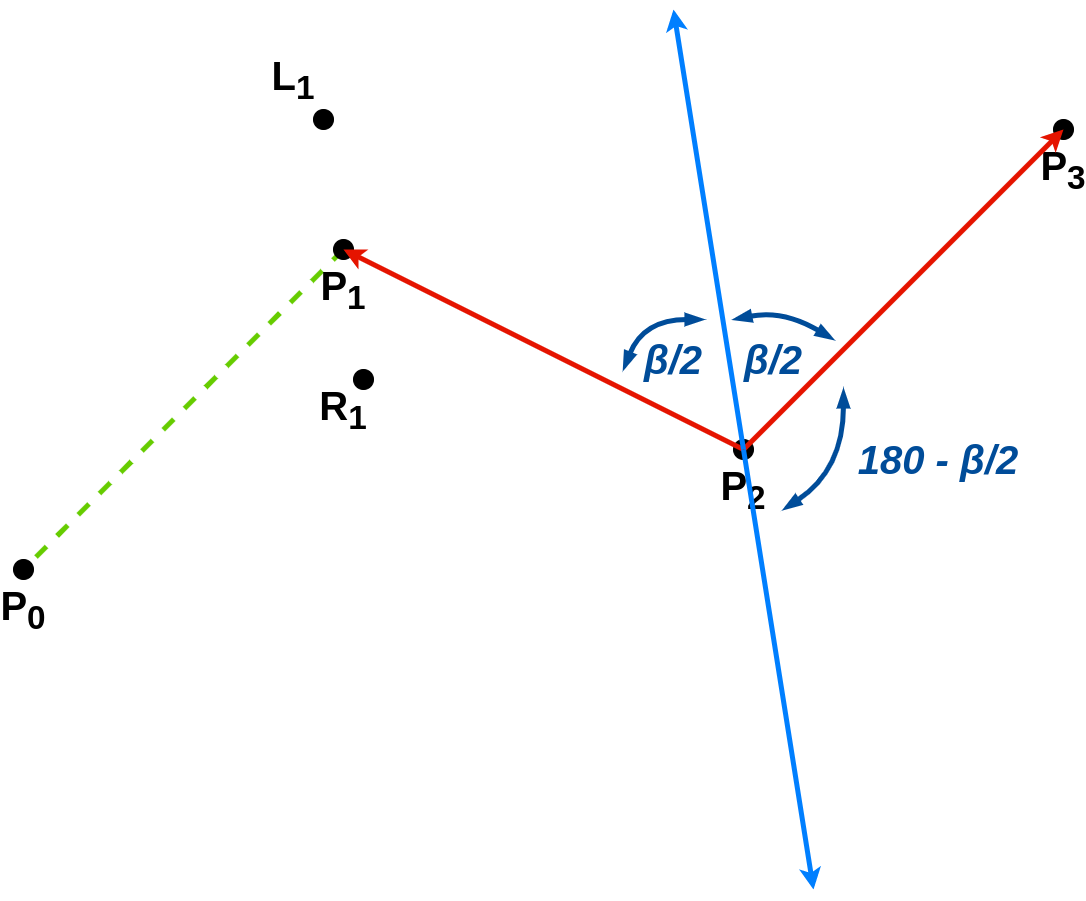
\includegraphics[width=1\linewidth]{Schlangenlinie-6.png}
        \caption{Schritt 6}
    \end{subfigure}
    \qquad
    \begin{subfigure}[b]{0.35\textwidth}
        \centering
        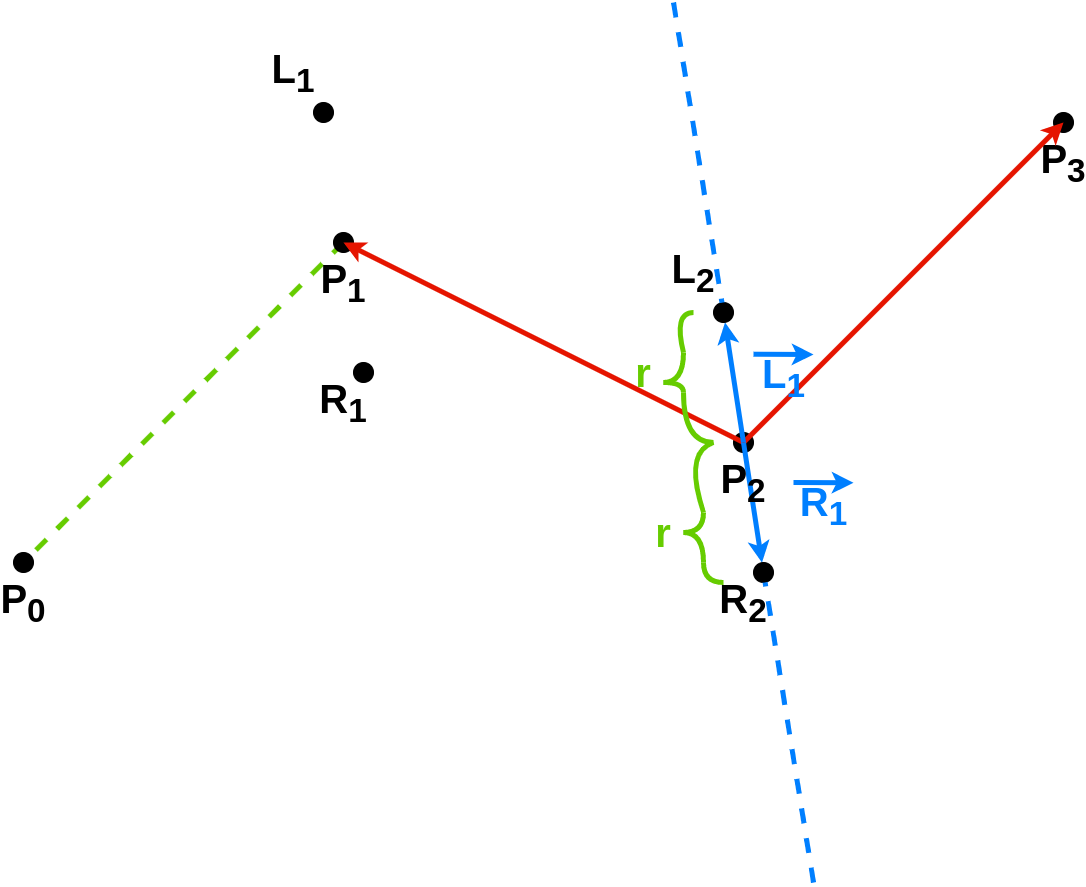
\includegraphics[width=1\linewidth]{Schlangenlinie-7.png}
        \caption{Schritt 7}
    \end{subfigure}
    \qquad
    \begin{subfigure}[b]{0.35\textwidth}
        \centering
        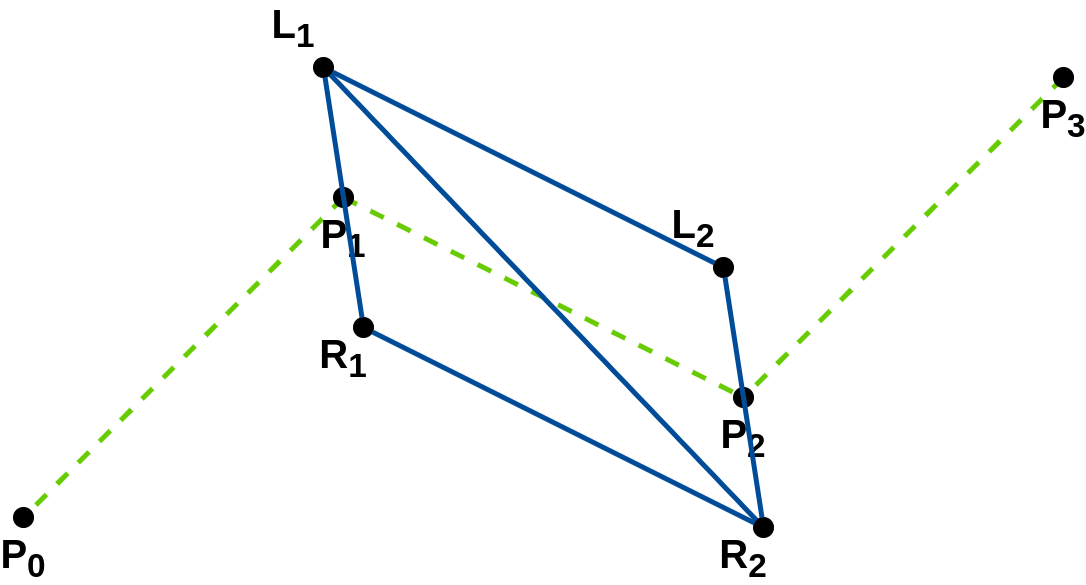
\includegraphics[width=1\linewidth]{Schlangenlinie-8.png}
        \caption{Schritt 8}
    \end{subfigure}
    \caption{Beispiel der Erzeugung eines Linien-Segmenten}
	\label{fig:line}
\end{figure}

\section{Bewegung}

\subsection{Startgeschwindigkeit}

Alle \textit{PlayerModel}s starten mit dem gleichen 
Geschwindigkeitsvektor $v$.

\begin{equation}
    v =
    \begin{bmatrix}
        0.09    \\
        0
    \end{bmatrix}
\end{equation}

Wenn ein Player initialisiert ist, wird ein randomisierten Winkel $\theta$ 
erzeugt. Anschließend wird der Vektor $v$ in z rotiert, um einen neuen Vektor zu 
erzeugen.

\begin{equation}
    \begin{bmatrix}
        v'_{x} \\
        v'_{y}     
    \end{bmatrix}
    =
    \begin{bmatrix}
        cos(\theta) & -sin(\theta) \\
        sin(\theta) & cost(\theta)
    \end{bmatrix}
    \begin{bmatrix}
        v_{x} \\
        v_{y}
    \end{bmatrix}
    \label{eq:rotation}
\end{equation}

Der Vektor $v$ wird durch $v'$ ersetzt.

\subsection{Im laufenden Spiel}
In jedem Frame gibt es 3 Fälle für alle aktiven Player:

\paragraph{Der Player drückt keine Steuerungstaste}
Der Geschwindigkeitsvektor $v$ bleibt gleich und der Player bewegt sich
in die gleiche Richtung.

\paragraph{Der Player drückt die linke/rechte Taste}
Der Geschwindigkeitsvektor $v$ wird wie in der Gleichung \ref{eq:rotation}
rotiert.

\paragraph{Der Player ist tot}
Der Player wird nicht mehr geupdated, der Geschwindigkeitsvektor bleibt gleich
aber er wird sich nicht bewegen.

\section{Kollisionen}

Vereinfachend werden alle Punkte der Linien als Kreisen betrachtet.
Da alle Elementen im Spiel als Kreisen betrachtet werden, kann man eine Kollision
detektieren, wenn der Abstand zwischen beiden Kreisen kleiner als die Summe ihrer Radien sind.

Seien $C_{1}$ und $C_{2}$ die Zentren zweier Kreise. Der Abstand zwischen den 
Zentren wird mit der folgenden Gleichung gberechnet:

\begin{equation}
    d = \sqrt{(C_{1x} - C_{2x})^2 + (C_{1y} - C_{2y})^2}
\end{equation}

\begin{figure}[!htb]
    \centering
    \begin{subfigure}[b]{0.45\textwidth}
        \centering
        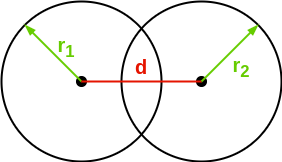
\includegraphics[height=0.1\textheight]{collisions-3.png}
        \caption{$d < r_{1} + r_{2}$}
    \end{subfigure}
    \qquad
    \begin{subfigure}[b]{0.45\textwidth}
        \centering
        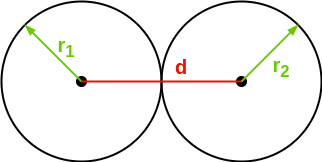
\includegraphics[height=0.1\textheight]{collisions-4.png}
        \caption{$d = r_{1} + r_{2}$}
    \end{subfigure}
    \qquad
    \begin{subfigure}[b]{0.45\textwidth}
        \centering
        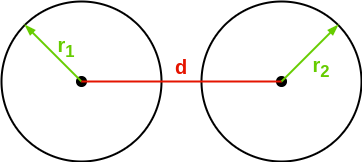
\includegraphics[height=0.1\textheight]{collisions-5.png}
        \caption{$d > r_{1} + r_{2}$}
    \end{subfigure}
    \caption{Fälle für die Kollisionen}
    \label{fig:collisions-1}
\end{figure}

\FloatBarrier
In jedem Frame wird der Abstand zwischen jedem Player und jedem Punkt,
sowie der Abstand zwischen jedem Player und dem Border berechnet. 
Der Prozess ist in der Abb. \ref{fig:collisions-2} dargestellt.

\begin{figure}[!htb]
    \centering
    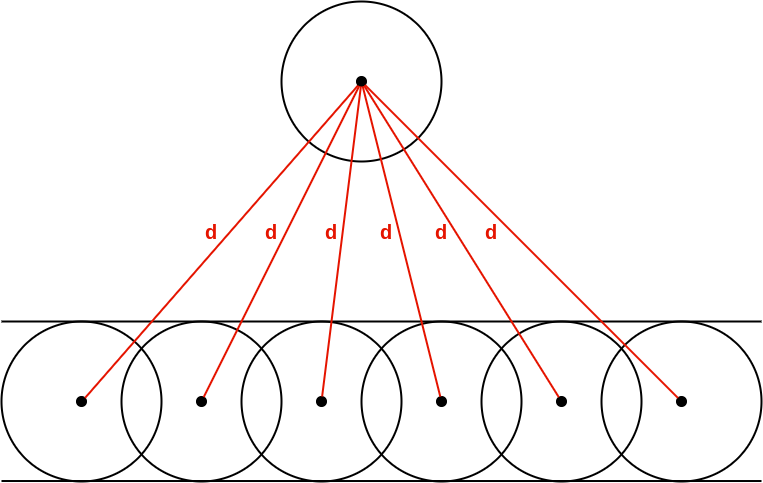
\includegraphics[width=0.6\linewidth]{collisions-2.png}
    \caption{Der Player überprüft seinen Abstand mit allen Punkten in den Linien}
    \label{fig:collisions-2}
\end{figure}

\section{Projektdokumentation}

Für die Entwicklung des Projektes wurde die IDE Visual Studio Code (VSCode) 
ausgewählt. VSCode besitzt ein kostenloses Pluging, welches das Pair Programming
erlaubt, das LiveShare heißt. Im Kombination mit Skype konnte das Projekt
gleichzeitig entwicklen werden.

Für den Code wurde ein Github Repository erstellt, welches es erlaubt hat,
asynchron zu arbeiten.

\section{Benutzerhandbuch}

\subsection{Installation}
Das Projekt befindet sich in GitHub auf dem Repository 
\url{https://github.com/h-valdes/kurve}. \\

Installieren Sie die Dependencies:
\begin{enumerate}
    \item GLFW
    \item FreeType2
\end{enumerate}

Clonen Sie das Repository:
\begin{lstlisting}[language=bash]
$ git clone https://github.com/h-valdes/kurve.git
\end{lstlisting}

Estellen Sie einen neuen Build Ordner auf dem Ordner des Repository und 
kompilieren Sie das Projekt:
\begin{lstlisting}[language=bash]
$ mkdir build
$ cd build
$ cmake ..
$ make
\end{lstlisting}

Um das Projekt zu starten:
\begin{lstlisting}[language=bash]
$ ./kurve
\end{lstlisting}

\FloatBarrier
\subsection{Spielanweisungen}

Es gibt 6 mögliche Spieler. Jeder Spieler hat 2 vordefinierten Steuerungstasten:

\begin{table}
    \centering
    \begin{tabular}{ |c|c|c| }
        \hline
        Name & Links & Rechts \\
        \hline
        Gryffindor & L.Ctrl  & L.Alt \\
        Slythering & 1       & Q \\
        Hufflepuff & M       & , \\
        Ravenclaw  & L.Arrow & R.Arrow \\
        Muggle     & O       & P \\
        Squib      & B       & N \\
        \hline
    \end{tabular}
    \caption{Steuerungstasten der Spieler}
\end{table}

\FloatBarrier
Um das Spiel zu starten, müssen mindestens 2 Spieler ihre Anwesenheit 
bestätigen. Die Bestätigung wird mit ihrer respektiven linken
Steuerungstaste durchgeführt. Zum abbrechen muss die rechte Steuerungstaste 
gedrückt werden. \\

Wenn nur ein Spieler übrig ist, wird die Runde beendet. Der Name des Gewinners
blinkt kurz und nach dem Blinken kann die nächste Runde mit der 
SPACE-Taste gestartet werden. \\

Wenn ein Spieler die maximale Punktzahl erreicht hat, ist das Spiel zu Ende.

\printbibliography[heading=bibintoc]

\newpage
\appendix
\section{Screenshots}
\begin{figure}[!htb]
	\centering
	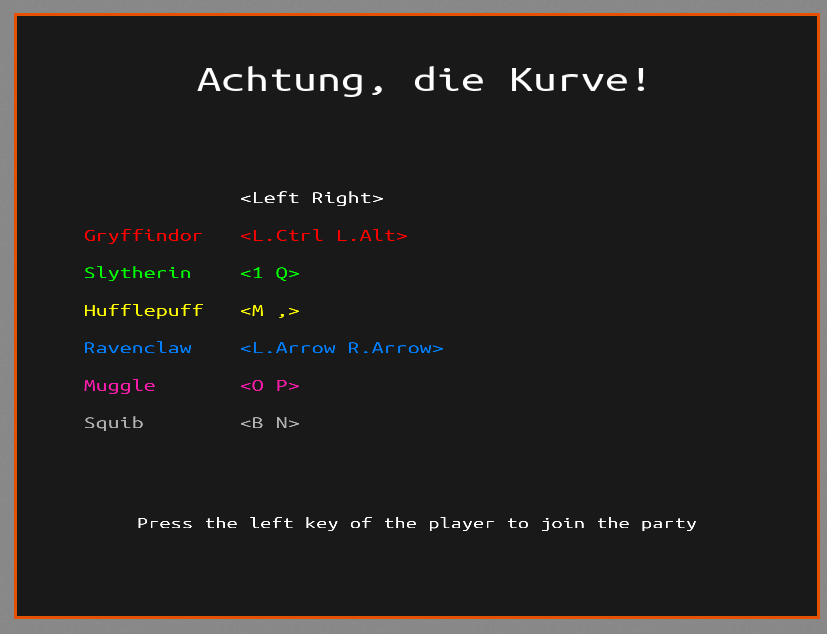
\includegraphics[width=0.9\linewidth]{1.png}
	\caption{Menü Szene.}
	\label{fig:menu}
\end{figure}

\begin{figure}[!htb]
	\centering
	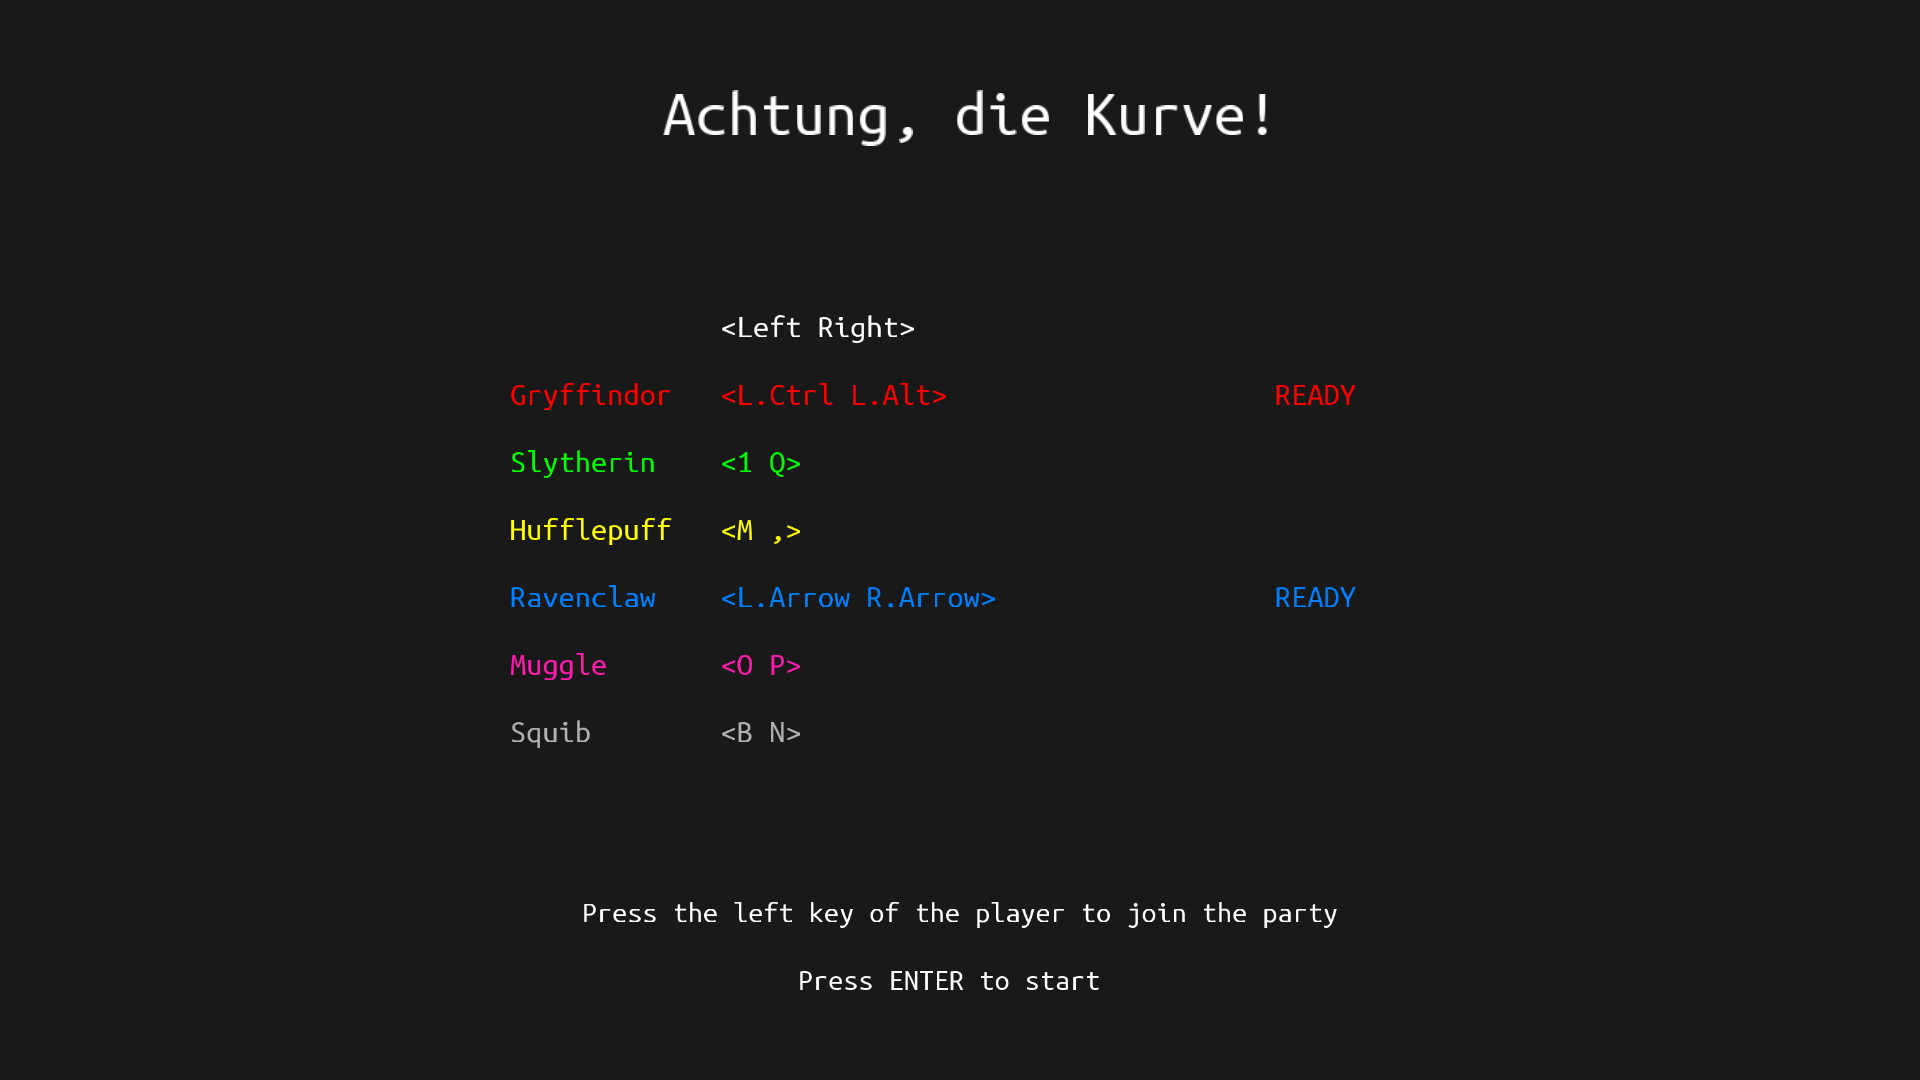
\includegraphics[width=0.9\linewidth]{2.png}
	\caption{Bestätigung der Anwesenheit von Spieler.}
	\label{fig:confirmation}
\end{figure}

\begin{figure}[!htb]
	\centering
	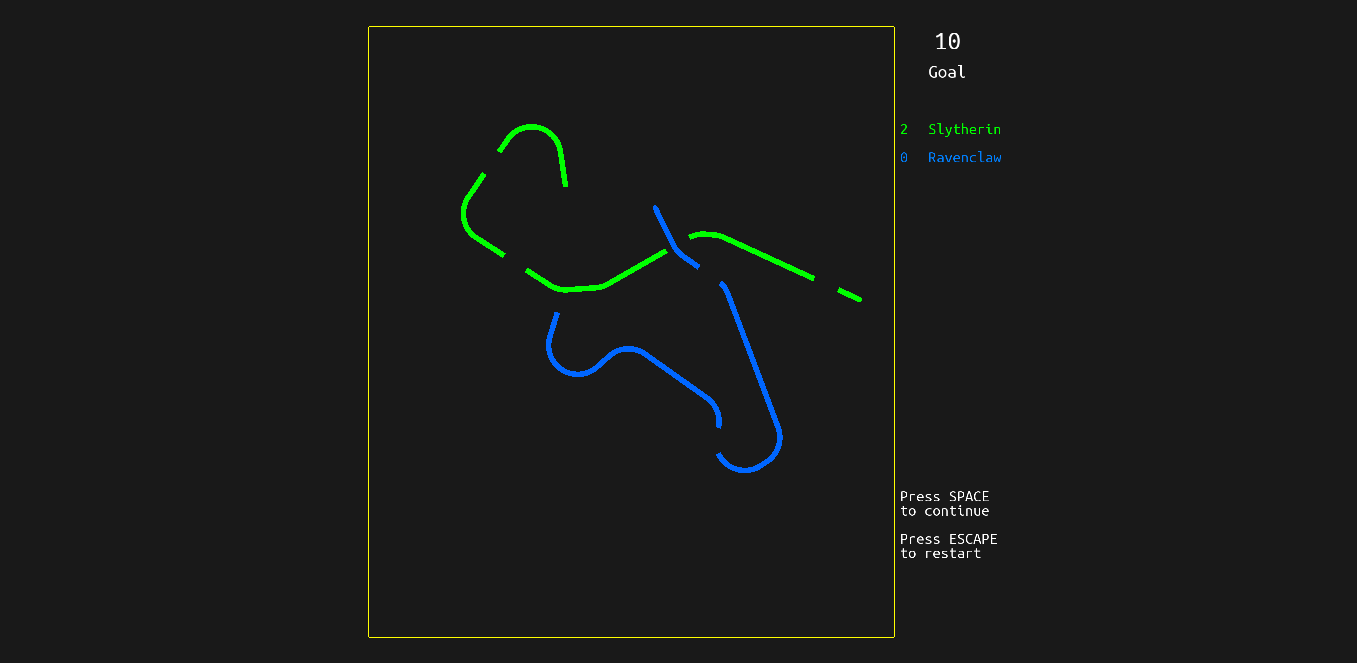
\includegraphics[width=0.9\linewidth]{3.png}
	\caption{Ein Spiel pausiert.}
	\label{fig:pause}
\end{figure}


\end{document}